\newpage

\section{The Transformation Protocol}

\genHeader

In Part IV, Section 6, we introduced the integrator feature which allows you to visually trace a transformation between two models. It's based on the
correspondence or link metamodel, but actually runs off the relevant \texttt{protocol.xmi} file. This file essentially provides the exact same information as
the integrator, but in much deeper detail. Don't worry -- it's not as scary as it looks!

To help us explain, let's compare what we see using the intergrator with \texttt{corrFWD.xmi} and \texttt{protocol\_FWD.xmi}, as generated at the end of the
introduction to Part IV, Section 7, where a fourth partition and card was added to \texttt{source.xmi} before we added a rule to handle it.

First, check out in integrator in Fig.~\ref{eclipse:integratorFWD}.

\begin{figure}[htbp]
\begin{center} 
  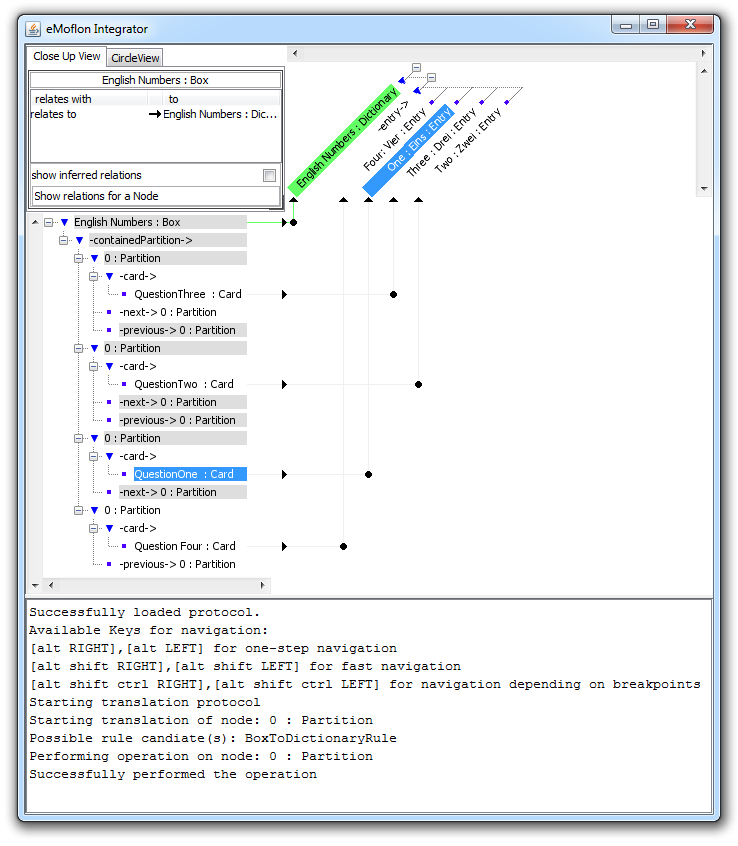
\includegraphics[width=\textwidth]{eclipse_integratorFWD}
  \caption{comment}  
  \label{eclipse:integratorFWD}
\end{center}
\end{figure}

It starts the transformation from :::

Now let's see the equivalent steps in the protocol file, described in Fig.~\ref{eclipse:protocolFWD}.

\begin{figure}[htbp]
\begin{center} 
  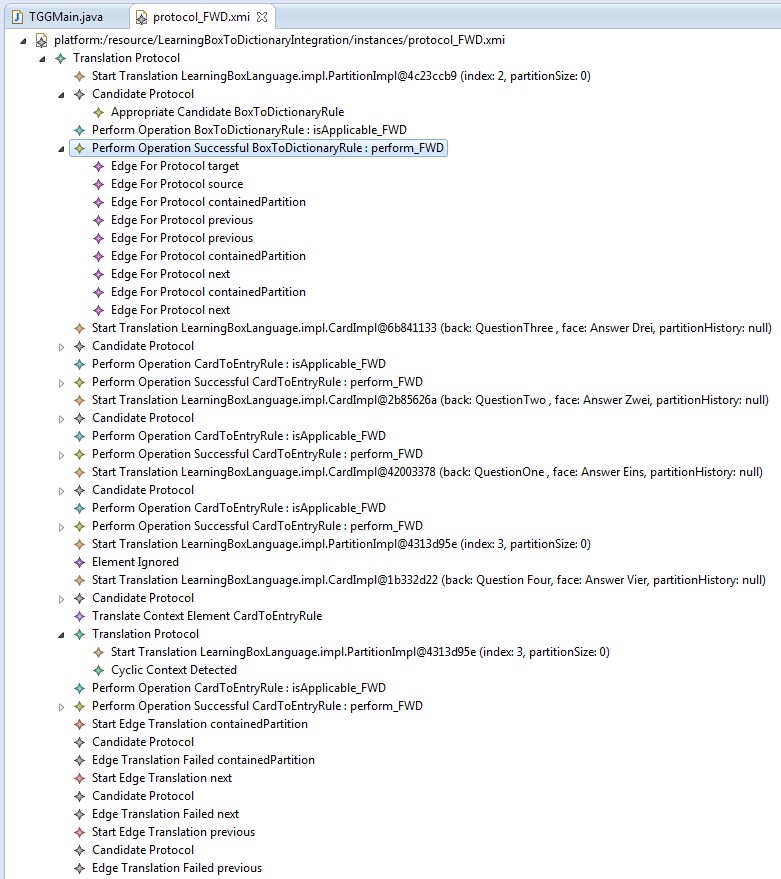
\includegraphics[width=\textwidth]{eclipse_protoFWD}
  \caption{comment}  
  \label{eclipse:protocolFWD}
\end{center}
\end{figure}

Again, it starts by trying to translate \ldots It's obvious that every edge listed under the successful operation procedure are the colourful and visualized
elements in the integrator.

Let's skip ahead to the expanded translation protocol, which is the beginning of out ``errors'' First, 5 titles above it, you'll notice it says ``Element
ignored''. Double clicking on that, we can see Fig.~\ref{eclipse:ignoredElement} that it ignored partition 3. you'll notice that this cyclic error is because
the translation was following the exact same steps. So instead, it just goes ahead and applies \texttt{cardToEntry} anyway (optimistic).

\begin{figure}[htbp]
\begin{center} 
  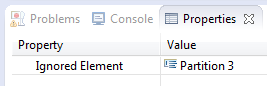
\includegraphics[width=0.5\textwidth]{eclipse_ignoreElementProperty}
  \caption{comment}  
  \label{eclipse:ignoredElement}
\end{center}
\end{figure}

Finally, it tries to translate the only remaining element, \texttt{containedPartition}. You'll notice that there is nothing under `Candiaite protocol' Clicking
on the `edge translation failed,' instead of being stuck guessing like we would have in the integrator (image?), the properties tell us exactly what the problem
is - there's no rule able to handle this! (Fig.~\ref{eclipse:NoAppRule})

\begin{figure}[htbp]
\begin{center} 
  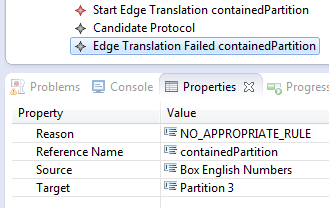
\includegraphics[width=0.5\textwidth]{eclipse_NoAppRule}
  \caption{comment}  
  \label{eclipse:NoAppRule}
\end{center}
\end{figure}

Conclusion
